% $Id: gmmf.tex,v 1.26 2008/05/04 10:37:19 Moritz.Ringler Exp $ 
% Kein unabhaengiges LaTeX-Dokument! 
% Master-Dokument: diss.tex  
%
\section{GMM -- a Generalized Mie Scattering code}\label{app.gmmf}

The program GMM \cite{gmm01f} by Yu-Lin Xu implements Generalized Mie Scattering
according to \cite{xuy95, xuy95err, xuy97, xuy98}. The main difference from
the treatment in these articles is the use of another normalization constant $\emn$. Details
about this and a general introduction to GMM can be found in the original GMM
documentation distributed together with GMM.

For a given aggregate of spherical nanoparticles, GMM\index{GMM} calculates the
scattering, extinction and absorption cross sections\footnote{GMM also 
calculates the scattering matrix, but this is of no importance in the context
of GMM-DIP and GMM-FIELD.} for an incoming plane wave of a given wavelength.
The overall program flow is represented in figure~\ref{abb.gmm}.

\begin{algorithm}[h]
\KwData{$n_\mathrm{max}$, $\lambda$, $N$; $\vec{r}^\beta$, $R^\beta$, $\epsint^\beta$}
\KwResult{\cro{str}, \cro{ext}, \cro{abs}}
\Begin{
read wavelength\;
read aggregate parameters\;
calculate Mie coefficients for all spheres\;
calculate vector translation coefficients\;
expand the incoming wave in vector spherical harmonics $\rightarrow p_{mn}^{0\;\beta}, q_{mn}^{0\;\beta}$\;
calculate scattering coefficients for all spheres $\beta$ $\rightarrow a_{mn}^\beta, b_{mn}^\beta$\;
calculate scattering cross section\;
calculate extinction and absorption cross sections\;
output\;
}
\caption{Program flow of GMM}\label{abb.gmm}
\end{algorithm}

GMM has no external dependencies and can be compiled with the FORTRAN compilers
of the GNU Compiler Collection,
%\footnote{\uri{http://gcc.gnu.org/}}%
gfortran and g77, on all platforms where these are available. 
For \cite{phdrin08}, I used gfortran (gcc~4.2.1) under SUSE Linux and
g77 (gcc~3.4.4) under Windows/Cygwin.
%\footnote{\uri{http://cygwin.com}}. 
GMM and the commercial MQAggregates \cite{qui93}
will produce identical results when given the same input.
GMM is usually faster and easier to control from the shell,
which makes it possible to write shell scripts that
automatically calculate a series of scattering spetra e. g. for
different particle distances in a dimer.

\clearpage{}
\ifhyperref{\phantomsection}{}
\section{GMM-FIELD -- a GMM Extension that Calculates the Near Field}\index{GMM-FIELD}
To understand nanoparticle dimer resonators and to calculate fluorescence and
Raman scattering in their interior, as in \cite{rin08}, one must know the
local electric field. The original GMM calculates only far field quantities,
but it can be extended in such a way that the near field is also obtained.
GMM-FIELD is such an extension.
%
\footnote{The source code of GMM-FIELD  as well as some example applications
can be downloaded from
\mbox{\uri{http://moritz-ringler.name/dissertation/GMM\_FIELD.tar.bz2}}.}

The local field in the space 
$\mathcal{A}$ outside the particles is given by the sum
$\evec = \einc + \escat$. 
The incident field \einc{} is trivially calculated for a plane wave
as $\exp{i k z}\;\ex$. The scattered field $\escat$ can be calculated with
either of two approaches: you can expand the 
scattered field of all spheres in the vector spherical harmonics of one 
particular sphere (or another point in space) and evaluate this expansion
for all the points of the grid $G$ on which you want to know the field.
Alternatively, you can transform the cartesian coordinates of each grid point 
into the spherical coordinate systems of each sphere $\beta$, 
calculate the partial 
scattered fields $\escat^\beta$ in those coordinate systems,
and finally sum them in the original cartesian coordinate system.
I have chosen this latter approach for GMM-FIELD.
The algorithm of the routine that has been added to 
GMM in GMM-FIELD to obtain the local electric field is schematically represented
in figure~\ref{abb.gmmfield}.

\begin{algorithm}[ht]
\KwData{$\lambda$, $\beta_\mathrm{max}$, $n_\mathrm{max}$, $\vec{r}^\beta$, $R^\beta$;
$a_{mn}^\beta$, $b_{mn}^\beta$;
$G$}
\KwResult{$\evec(x, y, z)$ for all $(x, y, z) \in\ G\ \cap \mathcal{A}$}
\Begin{
    Read grid definition from grid.in $\rightarrow G$\;
    {\color{darkblue}Calculate normalization factors $\rightarrow \emn{}$}\;
    \ForAll{$(x, y, z) \in G$}{
        $\evec = (\exp{i k z}, 0, 0)$\;
        \tcp{to calculate just the scattered field:}
        \tcp{$\evec = \vec{0}$}
        \For{$1 \le \beta \le \beta_\mathrm{max}$}{
            Calculate in spherical coordinates $\bigl((x, y, z) - \vec{r}^\beta\bigr)$
            $\rightarrow (r, \varphi, \theta)$\;
            \If{$r \le R^\beta$}{
                \tcp{Set the field in the interior of the spheres to zero.}
                $\evec = \vec{0}$\;
                break;
            }
            {\color{darkblue}Calculate vector spherical wave functions
            $\mmn{3}(\lambda, r, \varphi, \theta),\ \nmn{3}(\lambda, r, \varphi,
            \theta)$}\;
            Calculate the partial scattered field $\rightarrow \escat^\beta$\;
            {\color{darkblue}Calculate cartesian components of the partial scattered field}\;
            $\evec = \evec + \escat^\beta$
        }
        Write $x$ $y$ $z$ $\Re(E_x)$ $\Im(E_x)$
            $\Re(E_y)$ $\Im(E_y)$ $\Re(E_z)$ $\Im(E_z)$
            $\|\evec\|$ to field.dat
    }
}
\caption{Local field routine in GMM-FIELD}\label{abb.gmmfield}
\end{algorithm}

The steps marked in blue are implemented as new subroutines.
For the other steps, existing subroutines of GMM have been reused or they
are implemented in the field routine itself. 
The main effort goes into calculating the vector spherical wave functions
$\mmn{3}$ and $\nmn{3}$,
because the special functions
$\pimn$, $\taumn$, $\pmn$,
$h^1_n$ and the derivative
$\diff{z}\left(z\, \func{h_n^1}{z}\right)$
must be evaluated for all $m$ and $n \le n_{\mathrm{max}}$
for each field point and each sphere.
Fortunately, existing GMM subroutines could be used for $\pimn$, $\taumn$ and 
$h^1_n$. The derivative $\diff{z}\left(z\, \func{h_n^1}{z}\right)$ 
is obtained by applying identity 10.1.21 from \cite{BookAbr64}
\begin{equation}
\diff{z}\left(z\, \func{h_n^1}{z}\right) = z\, \func{h^1_{n-1}}{z} - n\, \func{h^1_n}{z}
\end{equation}
The associated Legendre functions $\pmn$ are calculated for $m \ne 0$ according
to:
\begin{equation}
m\, \pmn(z) = \pimn(z) \sqrt{1 - z^2} \qquad \text{for} \quad z = \cos{\theta}
\end{equation}
$P^0_n$ is given by recursion 8.5.3 from~\cite{BookAbr64}
\begin{equation}
(n-m+1)\, P^m_{n+1}(z)
=
(2n+1)\,z\, P^m_{n+1}(z)
-
(n+m)\, P^m_{n-1}(z)
\end{equation}
together with $P^0_0(z) = 1$ and $P^0_1(z) = z$. 
For consistency with the rest of GMM the $P^0_n$ thus obtained
have to be multiplied by the factor
$\sqrt{(2n + 1)/(n(n + 1))}$.

\subsection{Usage Example}
As an example of how GMM-FIELD is controlled we will now have a look at the
input files that I have used to calculate the field enhancement in the
interior of a dye-filled nanosphere enclosed between two gold nanoparticles
when the dimer resonator is excited in the longitudinal mode \cite{bek07}.
We are using microns as the global length unit.

Let us first have a look at the GMM input file gmm01f.in.
This file tells the program that the parameters of aggregate and incoming 
wave can be found in au-2s-532nm.k and that the vector wave function
expansions must not be
truncated at less than twentyfirst order\footnote{%
The compile time parameter np in gmm01f.par must be set to a value greater than
or equal to the largest minimum vswf order you intend to use.}. 
For an explanation of the other 
directives please refer to the GMM documentation. They can in general remain
unchanged. 

\begin{verbatim}
au-2s-532nm.k
1 1 1
0. 0. 0. 0. 0. 0.
0
0
0  10000
0.7 0.7 100 = iteration control
20 = minimum vswf order; must be <= np in gmm01f.par
1.d-20 1.d-10
0.
0. 0.
\end{verbatim}

The aggregate and field definition au-2s-532nm.k reads as follows
\begin{verbatim}
 0.532 = wavelength
 2 = number of spheres; <= nLp in gmm01f.par
 -0.05 0.0 0.01 0.03 0.5440 2.2304 = x1,y1,z1; R1; Re(n),Im(n) at 532 nm
  0.05 0.0 0.01 0.03 0.5440 2.2304 = x2,y2,z2; R2; Re(n),Im(n) at 532 nm
\end{verbatim}
Here, the wavelength, the number of particles\footnote{%
The compile time parameter nLp in gmm01f.par must be set to a value greater than
or equal to the largest number of spheres you intend to use.}, their center coordinates and radii,
and their complex refractive indices at the incident wavelength are specified.
Note that the origin of the coordinate system is chosen to coincide with the
center of our region of interest, i. e. with the center of the dye-filled sphere.
The program always uses an $x$-polarised wave that propagates
in the $+z$-direction. To study the longitudinal dimer mode we have
thus aligned the dimer axis with the $x$-axis.

If the refractive index of the environment is different from one you can take 
that into account by specifying the wavelength in the medium
$\lambda = \lambda_0 / \sqrt{\epsext(\lambda_0)}$ and by 
entering the complex refractive index of the particles 
$\sqrt{\epsint(\lambda_0)}$ in units of the refractive index of the medium
$\sqrt{\epsext(\lambda_0)}$. The section on GMM-DIP contains an example of this
procedure.

The third input file grid.in defines the grid on which you would like to
evaluate the field. 
\begin{verbatim}
101 101 101 = nx, ny, nz
-0.02 -0.02 -0.02 = x0, y0, z0
\end{verbatim}
The grid -- a regular rectangular grid -- is specified
by giving the number of points along each linear dimension in the first line
and the coordinates of one of its corners in the second.
The grid is always centered about the origin of the coordinate system.
This places no restriction on the geometry of the problem because you can 
always translate the particle coordinates such that the center of your region
of interest is in the origin of the coordinate system.
You use the same length units in line two of grid.in as those used for the
particle coordinates and wavelength.

Here, we are using a cubic grid with
$101 \times 101 \times 101 \approx 10^6$
points that extends from \val{-20}{nm} to \val{+20}{nm} in each dimension.

After running gmmfield, we calculate the total field enhancement from the
result file field.dat with the following short awk-script.
\begin{verbatim}
awk 'BEGIN {n=0; inte=0 ; inte2=0};
     $1*$1 + $2*$2 + $3*$3 <= 0.0004 {n++; inte+=$10; inte2+=$10*$10};
     END {print n, inte/n, inte2/n}' field.dat
\end{verbatim}
For each line in field.dat we here check whether the 
grid point lies in the interior of the dye-filled sphere.
If so, the absolute value of the field at that point (which would be one if there
were no particles) is added to  \texttt{inte} and its square is added to 
\texttt{inte2}. Furthermore, the counter \texttt{n} is incremented.
At the end the number of grid points inside the dye-filled sphere
\texttt{n}, the average field enhancement \texttt{inte/n}, 
and the average excitation enhancement \texttt{inte2/n}
are printed to standard output.

\subsection{Comparison with published MMP-results on field enhancement near
a single gold particle}\index{MMP}

\begin{figure}
\begin{center}
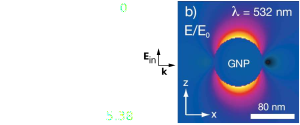
\includegraphics{abb/gmmhaertb}
\caption[GMM-FIELD, qualitative comparison with MMP results for a single particle]{
\textbf{GMM-FIELD, qualitative comparison with MMP results for a single particle.}
From the left a vertically polarised plane wave with
$\lambda = \val{532}{nm}$ 
hits a single gold particle with
$R = \val{40}{nm}$
in vacuum. The local field enhancement is shown, on the left calculated with
GMM-FIELD, on the right with MMP. MMP data are reproduced from
\cite{hae07}. The results are identical as far as this can be judged
given the different color maps. A legend for the color map is missing
from \cite{hae07}.
}\label{abb.gmmhaertb}
\end{center}
\end{figure}

We have checked whether GMM-FIELD is free of errors by trying to reproduce
the results on the field enhancement near a single gold nanoparticle that
have been obtained by H�rtling et al. with the multiple multipole method, 
MMP, \cite{hae07}.
The particle has a radius of \val{40}{nm} and is surrounded by vacuum.
It is hit by a plane wave with a wavelength of \val{532}{nm}. 
First, we will consider the field enhancement in the plane through the
center of the particle spanned by
\kvec{} and \einc{}. In \reffig{abb.gmmhaertb}, we see good qualitative
agreement between GMM-FIELD and MMP. A quantitative comparison is not
possible because the figure in \cite{hae07} has no legend for the color
scale.

\begin{figure}
\begin{center}
\includegraphics[width=\textwidth]{abb/gmmhaerta}
\caption[GMM-FIELD, quantitative comparison with MMP results for a single particle]{
\textbf{GMM-FIELD, quantitative comparison with MMP results for a single particle.}
Excitation enhancement $g_\mathrm{exc} =
|\evec \cdot \hat{\dip{}}|^2/|\einc \cdot \hat{\dip{}}|^2$ for a dipole
oriented radially (a) 
and tangentially (b) with respect to the surface of the gold nanoparticle.
Particle radius and wave lengths are the same as in
in \protect\reffig{abb.gmmhaertb}. The MMP results 
from \cite{hae07} are drawn with a red dashed line,
the results obtained with GMM-FIELD are shown as red circles.
The violet and green curves are H�rtling's results on the 
quantum efficiency and the total fluorescence enhancement and are not
of interest here (see \reffig{abb.gmmdiphaert}).
}\label{abb.gmmhaerta}
\end{center}
\end{figure}

However, the graphs on the excitation enhancement 
$\gamma_\mathrm{exc}$ in fig.~3 of
\cite{hae07} do lend themselves to a quantitative comparison of MMP and GMM-FIELD,
because the excitation enhancement is calculated as
$\gamma_\mathrm{exc} = |\evec \cdot \hat{\dip{}}|^2/|\einc \cdot \hat{\dip{}}|^2$.
We consider the two most important cases where the dipole is parallel to
the incident field \einc{}, and is oriented either radially or tangentially with respect
to the surface of the gold nanoparticle.
Both geometries and the respective results are
shown in 
\reffig{abb.gmmhaerta}. 
We see quantitative agreement. Small
deviations can be explained by differences in the dielectric function
used, the discretization error of the MMP calculation and 
numerical (i. e. rounding) errors.

